\section{System Description}
\subsection{System Modeling}

% Coba definisikan bentuk setup quadrotornya


We define the world frame as $\mathcal{W}$ and the body frame as $\mathcal{B}$, position is $\mathbf{r} = [x, y, z]^T$, and orientation is defined by Euler angles $\mathbf{\eta} = (\phi, \theta, \psi)$:

\begin{equation}
    \mathcal{W} = [x_{\mathcal{W}}, y_{\mathcal{W}}, z_{\mathcal{W}}],
\end{equation}

\begin{equation}
    \mathcal{B} = [x_{\mathcal{B}}, y_{\mathcal{B}}, z_{\mathcal{B}}].
\end{equation}

% \begin{figure}[htbp] 
%     \centering 
%     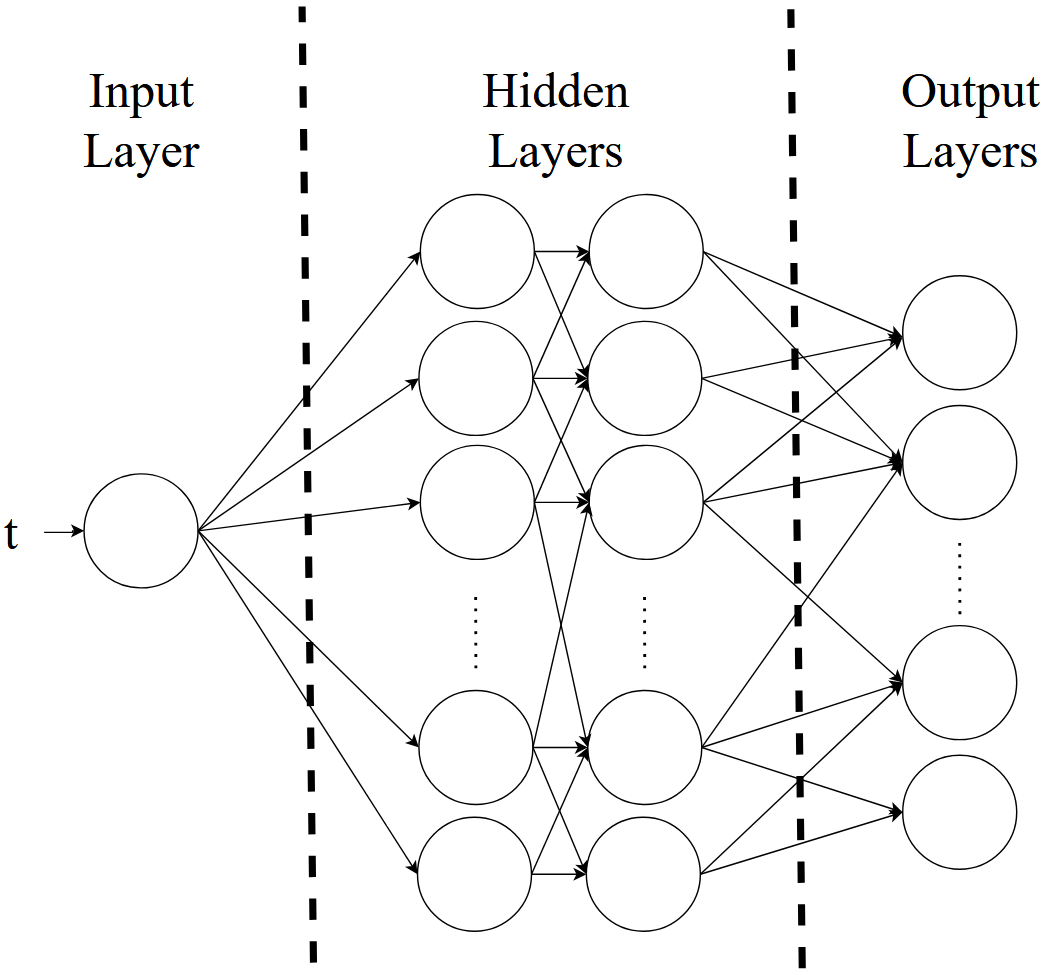
\includegraphics[width=0.3\textwidth]{images/pinns_architecture.png} 
%     \caption{Architecture of PINNs and the Multi-agent centralized control systems}
%     \label{fig:pinns_and_control_diagram} 
% \end{figure}

The MAS employs a centralized control architecture derived from \cite{mellinger2013trajectory}. The composite rigid body is commanded via a unified control wrench $\boldsymbol{\tau}$, defined as:

\begin{equation}
    \boldsymbol{\tau} = [F_B, M_{xB}, M_{yB}, M_{zB}]^T,
\end{equation}

\noindent where $F_B$ represents the total collective thrust acting along the inertial $z$-axis, while $M_{xB}$, $M_{yB}$, and $M_{zB}$ denote the respective desired roll, pitch, and yaw control moments applied about the body frame which relates to individual quadrotor thrust inputs $\mathbf{u} = [F_1, F_2, F_3, F_4]^T$ via the allocation matrix $A \in \mathbb{R}^{4 \times 4}$:

\begin{equation} \label{eq:tau}
    \boldsymbol{\tau} = [F_B, M_{xB}, M_{yB}, M_{zB}]^T = A \mathbf{u},
\end{equation}
\begin{equation}
    A =
    \begin{bmatrix}
        1 & 1 & 1 & 1 \\
        y_1 & y_2 & y_3 & y_4 \\
        -x_1 & -x_2 & -x_3 & -x_4 \\
        c_1 & c_2 & c_3 & c_4
    \end{bmatrix}.
\end{equation}

The rows of $A$ denote total thrust, roll moment, pitch moment, and yaw reactive torque, respectively. Required individual thrusts are derived by inversion:

\begin{equation}
    \mathbf{u} = A^{-1}
    \begin{bmatrix} F_B \ M_{xB} \ M_{yB} \ M_{zB}
    \end{bmatrix}\label{eq:inverse_allocation}.
\end{equation}

\subsection{Dynamic Thrust Allocation}
A payload shifts from the body central frame, altering the effective moment arms. Let $\hat{\mathbf{d}}_{\text{cog}} = [\hat{x}_{\text{cog}}, \hat{y}_{\text{cog}}]^T$ denote the estimated offset. Redefining the lever arms as $\Delta x_i = x_i - \hat{x}_{\text{cog}}$ and $\Delta y_i = y_i - \hat{y}_{\text{cog}}$, the allocation matrix adapts dynamically:

\begin{equation}
    A_{\text{final}} = \begin{bmatrix}
    1 & 1 & 1 & 1 \\
    \Delta y_1 & \Delta y_2 & \Delta y_3 & \Delta y_4 \\
    -\Delta x_1 & -\Delta x_2 & -\Delta x_3 & -\Delta x_4 \\
    c_1 & c_2 & c_3 & c_4
    \end{bmatrix}. \label{eq:allocation_matrix}
\end{equation}

Control inputs are computed via the Moore-Penrose pseudo-inverse to handle transient rank deficiencies:

\begin{equation}
    \mathbf{u} = A_{\text{final}}^{+} \boldsymbol{\tau}. \label{eq:final_u}
\end{equation}